\documentclass[8pt]{article}
\usepackage{graphicx}
\usepackage[utf8]{inputenc}

\title{Temporally equitable subsidies: a two-phase token minting schedule}
\author{arjunhassard}
\date{March 2020}
\begin{document}
\maketitle

\section{Summary}

We propose a two-phase subsidy model to bootstrap the NuCypher network, the first phase comprising a \textit{stable issuance}, in which approximately 366 million new tokens are minted and distributed to active (staking) node operators every year in the first phase, set to 5 years. This is equivalent to expanding the supply by 1,002,509 tokens in each of the first 1825 periods (days). In the second phase, commencing on the first period of the fifth year, fewer tokens will be minted in each successive period, such that the daily minting figure decays exponentially with a half-life of 2 years. Over the course of the network's lifetime – as $t$ approaches $\infty$ – the circulating supply will approach a maximum of roughly 3.885 billion tokens. 

\begin{figure}[h!]
    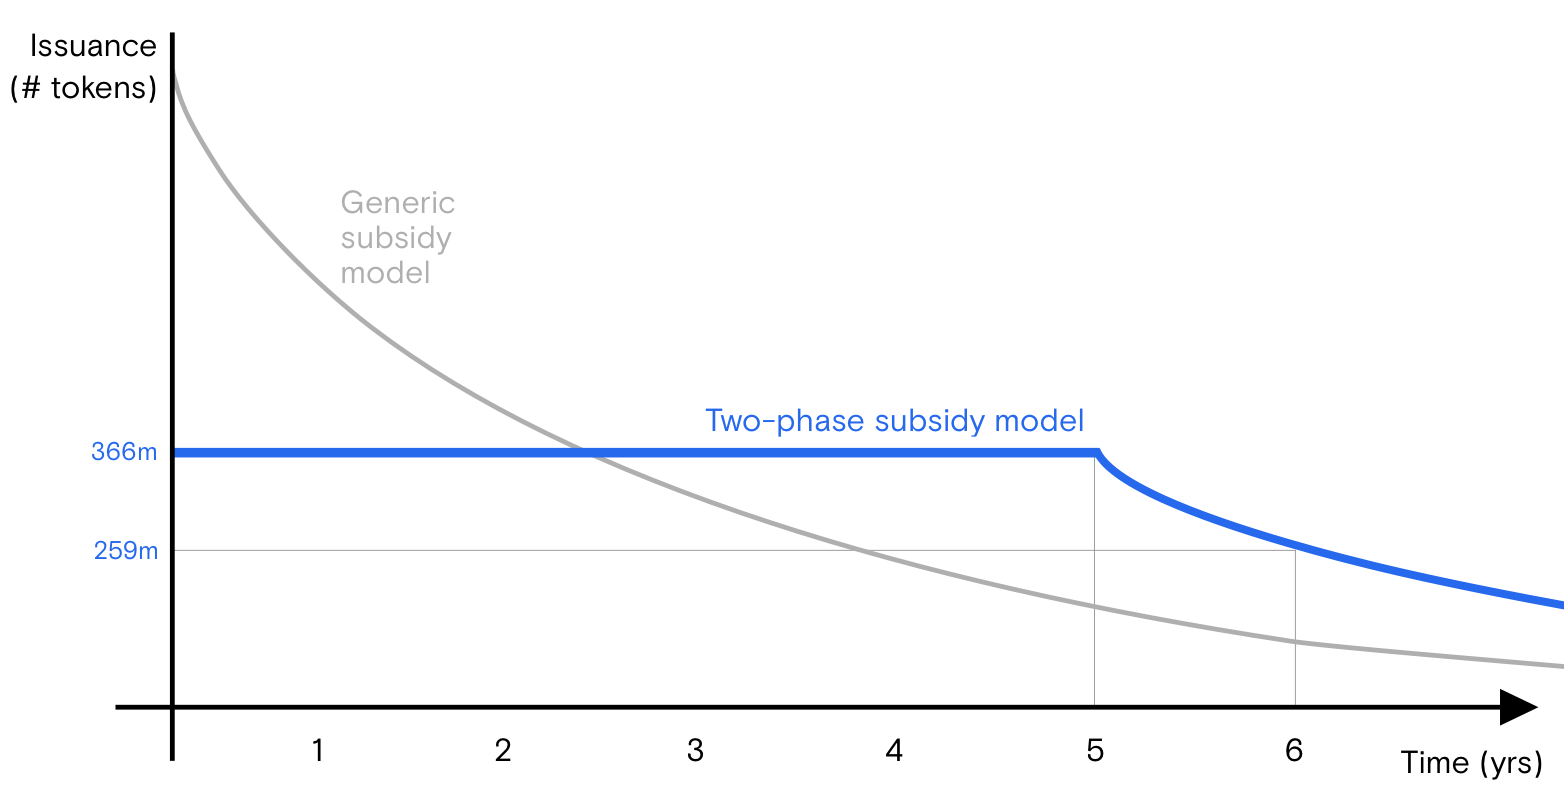
\includegraphics[width=\textwidth]{Two_phase_model.png}
    \caption{Illustration comparing a two-phase model with a common subsidy model, over the first 6 years of the network's lifetime. Note that the y-axis refers to an absolute figure, not a rate.}
    \label{fig:tp}
\end{figure}

Monetary policy designed for decentralized networks often make reference to a so-called `inflation rate'. In this model, phase one sees an \textbf{constant amount of tokens} minted in each period, so the effective `rate' at which the circulating supply grows decreases period-to-period (and year-to-year). In phase two, the number of tokens minted per day also decreases, which accelerates the decline in the supply growth rate. To avoid misleading terminology, the number of total tokens minted per day shall be hereafter referred to as the \textit{issuance}. Note that the effective growth rate of any given stake also decreases over time, the extent to which is subject to discretionary factors such as the percentage of tokens re-staked by the node operator. 
\\\\
In the NuCypher protocol, daily issuance is modified by the average stake lock-up duration, but for the sake of simplicity this paper initially discusses a scenario in which all node operators choose a lock-up of 12 months or longer. In reality, the average stake lock-up duration is likely to be lower, which would imply fewer tokens minted per day. This has an impact on the global economy and supply, but regardless, all node operators choose discretionary lock-up durations and receive commensurate subsidies.
\\\\
The second section introduces reasoning for the two-phase model pertaining to network demand, the protocol and node operation, the third introduces an empirical analysis of existing networks, and the final section derives parameters for the new minting schedule.

\section{Motivation \& Rationale}

\subsection{Demand uncertainty}

These demand-related premises form the basis for the two-phase model: 
\begin{enumerate}
\item There is little certainty regarding the length of time that will elapse between the network's launch and the development of meaningful demand from customers (developers, end-users \& others).
\item This early-stage demand is particularly fragile, because new customers are naturally more fickle. Specifically, neither developers nor their end-users have compelling reasons to tolerate an inadequate service (e.g. too few stakers available to service a sharing policy), such as the sunk costs of integration, reliance on the service, or other forms of path dependency, all of which are more likely to play a role later in the network's lifetime. New customers also take a greater risk than later adopters, as they do not have the experience of existing customers as evidence of a reliable or valuable service.
\item A popular subsidy model involves daily token issuance dropping exponentially, right from launch. If the fee market does not sufficiently mature in time to make up for the sharp reduction in earnings the early years of the network's existence, some node operations may be rendered entirely unsustainable. 
\item Most importantly, some of NuCypher's early customers may (inflexibly) require long-lasting sharing policies. This means that the protocol must motivate the successive re-commitment to long token lock durations (i.e. staking for 12+ months) by a sufficient population of node operators. A diminished subsidy issuance, in lieu of a mature fee market, may not be enough to incentivize this repeated and essential re-commitment. 
\end{enumerate}

\\\\
Hence this model attempts to mitigate the risk of \textbf{fledgling network demand coinciding with a disincentivized, dwindling or transient supply}. Note that these arguments do not involve strong claims about when (or if) network adoption will occur. Instead, it is the acknowledgement of uncertainty with respect to an adoption timeline that forms the core of the problem, and underpins the utility and advantage of a stable issuance phase as part of a two-phase minting schedule. 

\subsection{Impeding centralization}

A stable issuance in the first phase brings other benefits, including the partial mitigation of a centralizing dynamic suffered by many staking networks, in which larger node operators utilize subsidies to increase/consolidate control of the token supply, thanks to the allocation of tokens in proportion to stake size. Moreover, larger operators can re-stake a greater percentage of subsidies (not needing to convert as much to fiat to cover operational costs), precipitating a `rich-get-richer' dynamic. If token issuance is highest in the earliest days of the network, larger operators are granted an even greater head-start over new node operators who start staking in a later era, \textbf{the presence of whom provides the network with an important, long-term counter-balance against centralization}. Relatedly, an important rationale for the \textit{work token} model is the supposition that new node operators purchase the network's native token in order to stake and earn revenue. With a token issuance that decays from genesis, new operators are doubly disadvantaged – they must pay the market price to acquire tokens, plus they receive a diminished subsidy. 
\\\\
Hence, a two-phase minting schedule assists all would-be node operators who don't happen to stake right at network launch, but decide to do so at a later date. By addressing the temporal inequity of the previous draft, we impede problematic centralization trends.

\subsection{Risks to operational feasibility, incentives and pricing}

As mentioned, the two-phase model implies, relative to other subsidy models, a lower number of tokens minted on day one. This in itself confers further advantages to network health:  
\begin{itemize}
\item The greater the real-world value of the subsidy, the further from a fee-driven `reality' a node's set-up may be in economic terms (for example, in terms of operational efficiency). When subsidies eventually run out, node operators who are unable to adapt may cease operations, threatening general service availability or even reneging on existing commitments to users. Under a model with higher token issuance early on, these inefficient operators may control a substantial proportion of the circulating supply by this point. 
\item If subsidies are worth significantly more than the typical sum of transaction fees earned in the same period, then the incentive to earn those fees may be blunted. This is particularly problematic for the protocol if the node operator duty required to collect subsidies does not align well with the duty required to earn fees, and the reliability of the latter impacts overall service quality. 
\item High but decreasing subsidies may compel some node operators to offer an unsustainably cheap service, with the intention of raising prices later once subsidies dry up. Any developers and their end-users that have become reliant on the service, but are unable to afford the higher price point, may see their application/business thrown into jeopardy. The existence of this risk is a serious friction for would-be network adopters planning an integration and justifying the associated upfront costs and technical dependency.
\item In NuCypher's case, existing market prices for comparable services – key/secrets management and dynamic access control – are extremely low on a per-user basis. Profitability is generally achievable through high volume, which is a long-term endeavour. This business reality aggravates all three above issues described in this sub-section.
\end{itemize}

\section{Empirical analysis of existing networks}

\textit{Full analysis to be published. This section contains a summary of results so far and an interpretation with respect to the two-phase model.}
\\\\
\textbf{Adjusted Reward}: The actual earnings of active stakers accounting for dilution, at a given timestamp. A function of each network's nominal issuance (`inflation rate') and consequent minting schedule. Referred to elsewhere as the real yield.
\\
\textbf{Total staked}: The percentage of tokens staked out of the total circulating supply at a given timestamp. Referred to elsewhere as the staking rate or participation rate.
\\\\
In five prominent staking/PoS networks, the cross-correlation (Pearson correlation) between the an Adjusted Reward time series and the Total Staked time series was examined over various time-lags. The correlation is largely \textbf{negative} (Livepeer, Tezos), or is \textbf{too weak to be conclusive} (IRIS, SNX, Cosmos). In Livepeer's case, for example, it appears that when the Adjusted Reward by stakers goes down, the collective `reaction' tends to involve staking more tokens. This is not necessarily a causal relationship, but these results nonetheless challenge established ideas about staking behavior and protocol designs which attempt to balance the staking rate (in other words, the assumption is that there is a causal relationship in the opposite direction). When one institutes an increasing time-lag between the data entries, the correlations hold until approximately 5 days have elapsed (see Figure 2) between the Adjusted Reward and the Total Staked, where we assume the latter reflects the subsequent choice between staking more, unstaking/unbonding, re-staking, or doing nothing. We see negative correlations when the data is \textit{detrended} (not shown here), although they fade after about 3 days.

\begin{figure}[h!]
    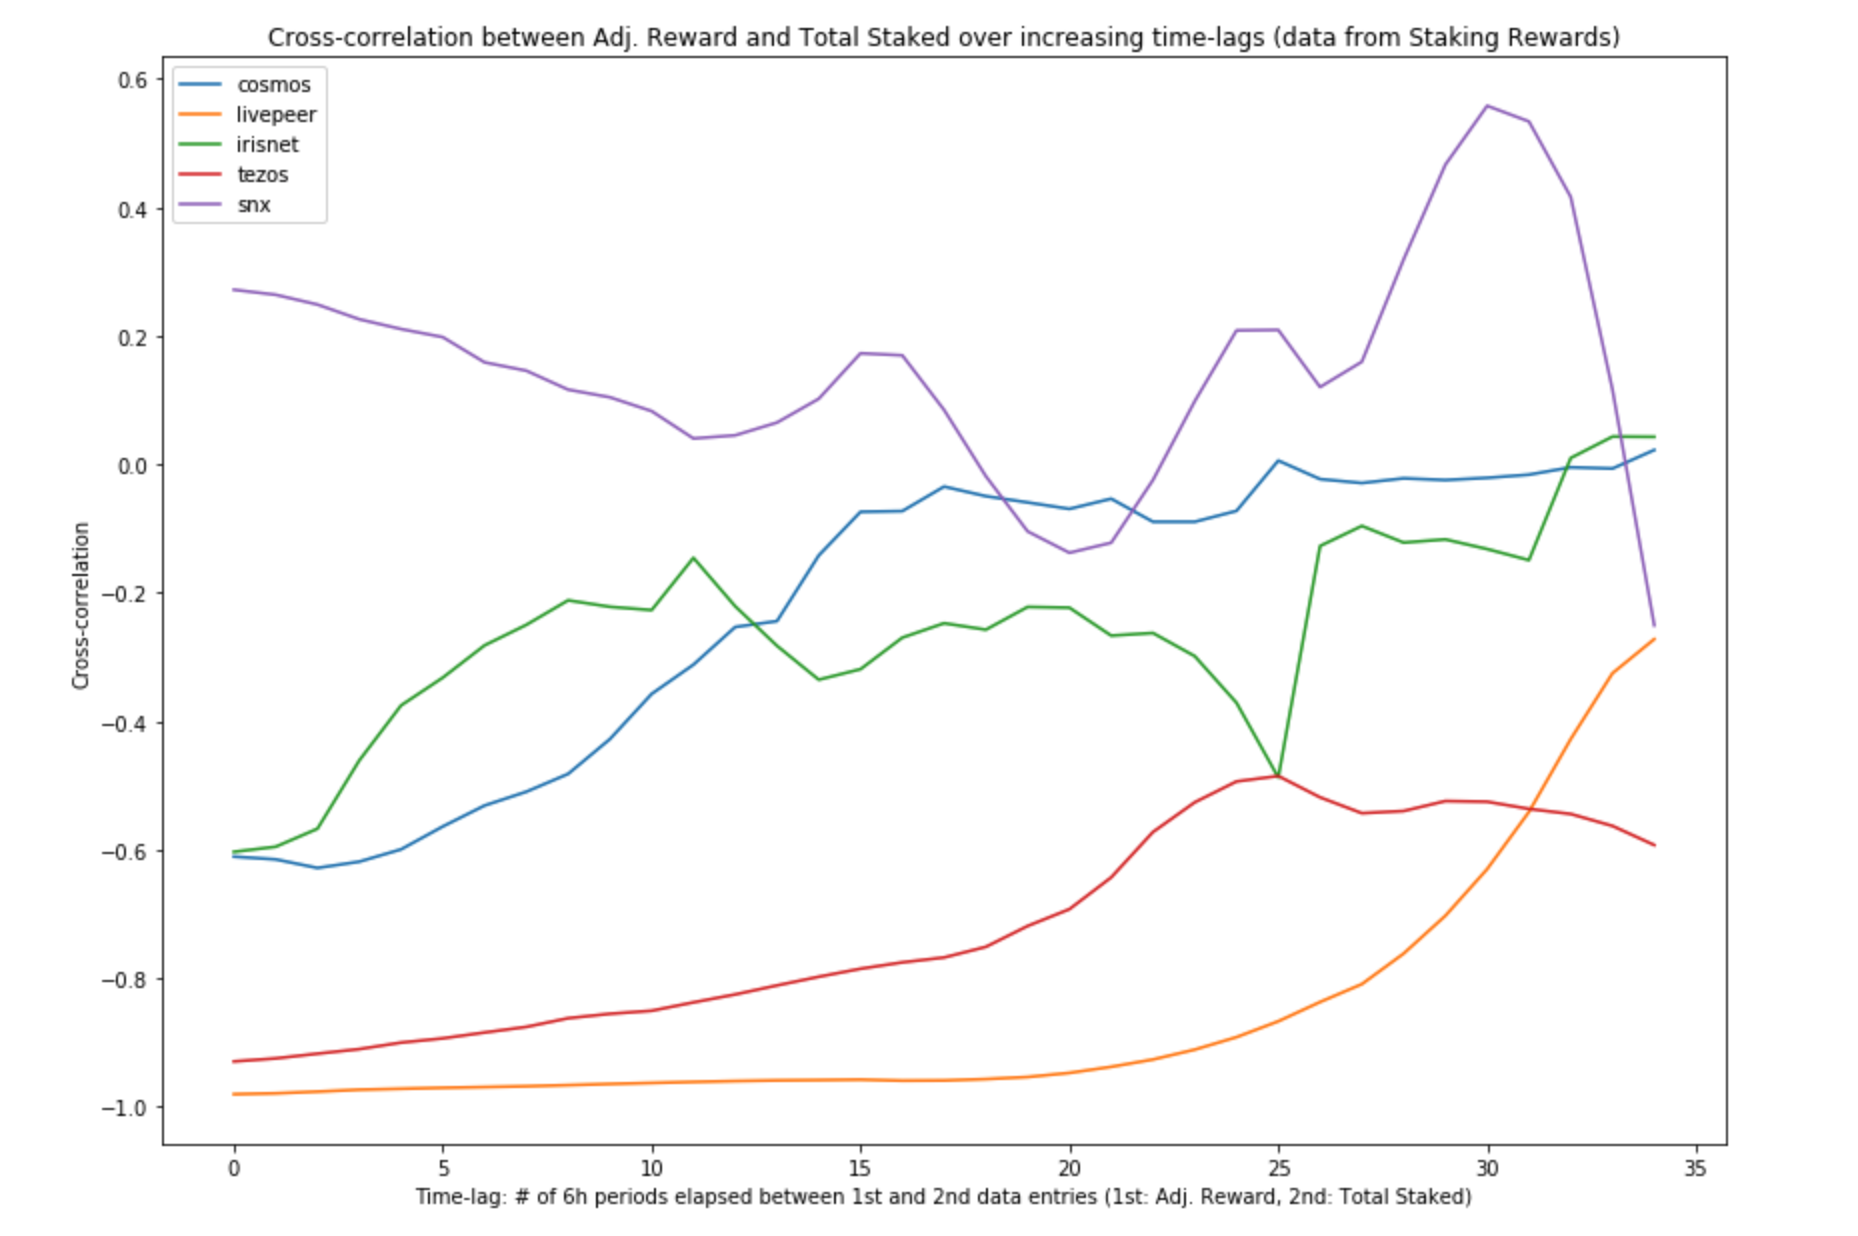
\includegraphics[width=\textwidth]{lagged_correlation_SR.png}
    \caption{Cross–correlation between Adjusted Reward and Total Staked over increasing time-lags. Data from Staking Rewards. N: [Cosmos: 1009, Livepeer: 1148, Irisnet: 1015, Tezos: 1371, SNX: 1005]. All five time series end in mid-February 2020.}
    \label{fig:tp}
\end{figure}

Thus, the notion that \textit{node operators can only be counted on for a reliable service if they're well compensated, or will quickly abandon the network} appears, so far, to be empirically false. None of the networks under examination, across multiple data set versions (from Staking Rewards and Staked Yields), have experienced a shortfall of operators, nor are there any observable trends that correlate decreasing earnings with a increasing paucity of supply, or increasing earnings with an increasing abundance of supply. There are multiple explanations for this, but none contradict the overarching rationale of the two-phase model. For example, one may study this seemingly unshakeable staker loyalty and tolerance of low reward rates, in the first year of these networks' existence and beyond, and attribute it to a prevalence of long-term investment strategies, deep pockets, ideological commitment or even irrational enthusiasm. Crucially, regardless of which underlying explanation you favour, there remains a strong case to flatten the minting schedule such that the earliest node operators do not capture a disproportionate share of the total supply.

\section{Deriving new parameters}

\\\\
In parametrizing the two-phase model, we fix certain parameters, and derive the rest from those constraints. We fix the total number of tokens ever to be minted, $S(\infty)$ at approximately 3.885 billion, and the half-life of the issuance decay in the second phase, $T_{1/2}$, at 2 years. We also fix the circulating supply at launch, $S_0$, at 1 billion tokens.

\subsection{Minting Schedule}
A key parameter for this model is the number of tokens minted per year in phase one, which we describe as the `stable issuance' ($I_{stable}$). Using an expression for $S(\infty)$, we can derive $I_{stable}$, expressible as a percentage of the genesis supply ($S_0$). $S(\infty)$ is the sum of (1) the tokens circulating at genesis, (2) the tokens minted in phase one, and (3) the tokens minted in phase two. Note that the boundaries of the second integral are $0$ and $\infty$, rather than $5$ and $\infty$, because the second phase exists mathematically \textit{as though} there was no first phase. Note also that all numerical figures in this derivation are rounded for readability.

\begin{equation}
    S(\infty) = S_0  +  S_0 \cdot \int_0^{5} I_{stable}(t)\, dt  +  S_0 \cdot \int_0^{\infty} I(t)\, dt
\end{equation}

For phase two, we calculate the decaying issuance at a time $t$.
 
 \begin{equation}
    I(t) = I_{stable} \cdot 2^{-\frac{t}{T_{1/2}}}
\end{equation}

We sub in $3.885 \cdot S_0$ for $S(\infty)$ and solve the first integral.

\begin{equation}
    3.885 \cdot S_0  = S_0 + S_0 \cdot (5 \cdot I_{stable}) + S_0 \cdot \int_0^{\infty} I_{stable} \cdot 2^{-\frac{t}{T_{1/2}}} \, dt
\end{equation}

We cancel out $S_0$ and solve the second integral.

\begin{equation}
    3.885 = 1 + 5 \cdot  I_{stable} + I_{stable} \cdot \left[\frac{-2^{(1-\frac{t}{2})}}{\ln{2}}\right]_0^\infty
\end{equation}

We are now able to find an expression for $I_{stable}$. Once again note that this variable is expressed as a percentage of the genesis supply, $S_0$.

\begin{equation}
    2.885 = I_{stable} \cdot (5 + \frac{2}{\ln{2}})
\end{equation}

\begin{equation}
   I_{stable} = \frac{2.885}{7.885} = 36.6\%
\end{equation}

We use $I_{stable}$ to find the number of tokens minted per year for the first 5 years.

\begin{equation}
   I_{stable} \cdot S_0 = 365,915,960\:\:new \:tokens \:per \:year
\end{equation}

This is equivalent to 1,002,509 newly minted tokens released into the circulating supply, every period (day) for the first 1825 periods. After this, the issuance decays on a period-to-period basis. For example, 1,001,558 tokens are minted on day 1827, which is 951 fewer than the previous day.
\\\\
In this token minting schedule, we can work out that approximately 1.83 billion tokens will be minted in the first phase, followed by a further 1.056 billion between the commencement of phase two and t = $\infty$.

\subsection{Variable stake lock-up duration}

In the NuCypher protocol, the number of tokens distributed to node operators in a given period depends on the stage in the minting schedule we are at and the size of their stake, but is also a function of the remaining duration their stake is locked up for (in fact, the duration of each of the `sub-stakes' they control). Any sub-stake locked up for a short duration receives less than the maximum subsidy, thereby slowing the expansion of the entire circulating supply – tokens are only minted if they are to be distributed to node operators. The number of tokens minted daily for a given sub-stake depends on the coefficient $\kappa$:

\begin{equation}
    \kappa &=& \left(0.5 + 0.5 \cdot \frac{\min(D_i, D_{max})}{D_{max}}\right)
\end{equation}

Where $D_i$ is the duration (the number of periods) until the sub-stake unlocks and $D_{max}$ is currently set to 365. 
\\\\
In phase one, a given sub-stake $i$ will have received the following sum of tokens by the period $p$.

\begin{equation}
    \label{eq:rate-max}
    ds_{i,p} = \kappa \cdot \frac{l_i}{L} \cdot \left(S_{P1} - S_{p-1} \right)\\
\end{equation}

Where $l$ is the size of the sub-stake, $L$ is the sum of all locked sub-stakes, and $S_{P1}$ is the maximum number of tokens to be minted in the first phase (approximately 1.83 billion tokens). In phase two, a similar equation can be utilized: 

\begin{equation}
    \label{eq:rate-max}
    ds_{i,p} = \kappa \cdot \frac{l_i}{L} \cdot \frac{\ln{2}}{T_{1/2}} \cdot \left(S_{P2} - S_{p-1} \right)\\
\end{equation}

Where $S_{P2}$ is the maximum number of tokens to be minted in the second phase (approximately 1.056 billion tokens). 
\\\\
The circulating supply at a given period is the sum of the tokens received thus far by all sub-stakes: 
\begin{equation}
    dS_p= \sum_i ds_{i,p},
\end{equation}

The implication is that it will likely take longer than 5 years to mint all the tokens reserved for phase one. The year in which the protocol switches from the first to second phase, $T_{1\rightarrow2}$, is therefore : 

\begin{equation}
    T_{1\rightarrow2}= \frac{S_{P1}}{S_0 \cdot \kappa^* \cdot I_{stable}}
\end{equation}

Where $\kappa^*$ is the average lock duration of all sub-stakes, weighted by relative size, across all periods in question. For example, if $\kappa^*$ is 73 days, then the minting schedule will switch phases about 8 1/3 years after network launch. If $\kappa^*$ is 11 months, $T_{1\rightarrow2}$ equals 5 years \& 79 days. 
\\\\
For reference, the supply in the second phase can be calculated with this equation: 

\begin{equation}
    S(t) = S_0 \left[1 + \frac{I_{stable} \cdot T_{1/2}}{\ln{2}}\left(1 - 2^{-\frac{t \cdot \kappa^*}{T_{1/2}}} \right) \right].
\end{equation}

Which implies that the rate of issuance decay is inversely proportional to $\kappa^*$. In a similar fashion to phase one, shorter average lock-ups slow down the minting of tokens. 

\end{document}
